%Sample for icsthesis.cls
%Author: JCEPlaras
%Reminders: Omit \lipsum commands

\documentclass{icsthesis}
\usepackage[english]{babel}

%\usepackage{showframe} %for debugging the margins
\usepackage{graphicx}
\usepackage{enumitem}
\usepackage{caption,float,adjustbox}
\usepackage[caption=false, font=footnotesize]{subfig}
\usepackage{natbib}

\usepackage{capt-of}  % <---
\usepackage{cuted}  
\usepackage{subfig}
\usepackage{multirow}
                              
                              
%Replace the values here, various commands depend on this variables                                                                                                                                                            
\renewcommand{\TITLE}{IDENTIFICATION OF GAN-GENERATED IMAGES THROUGH FREQUENCY ANALYSIS AND MACHINE LEARNING}
\renewcommand{\AUTHOR}{YANNA DENISE ALMODIEL HILARIO}
\renewcommand{\DEGREE}{BACHELOR OF SCIENCE}
\renewcommand{\MAJOR}{Computer Science}
\renewcommand{\MONTH}{APRIL}
\renewcommand{\YEAR}{2024}

\begin{document}
	
	\begin{frontmatter}
		%create title
		\maketitle
				
		\begin{approvalpage}
			The Special Problem hereto attached entitled \TITLE , prepared and submitted by \AUTHOR , in partial fulfillment of the requirements for the degree of \DEGREE\ (\MAJOR) is hereby accepted.
			
		\begin{multicols}{2}
				\centering
				%%\addsignature{Dr. VAL RANDOLF M. MADRID, PhD}{Member, Guidance Committee} %custom command for adding signature field
				%%\columnbreak
				%%\addsignature{RIZZA DC. MERCADO}{Member, Guidance Committee}
			\end{multicols}
			\addsignature{RODOLFO C. CAMACLANG III}{Chair, Guidance Committee}
            \\\\
			\par Accepted in partial fulfillment of the requirements for the degree of \DEGREE\ (\MAJOR). 
            \\\\
			\addsignature{Dr. MARIA ART ANTONETTE CLARIÑO, PhD}{Director, Institute of Computer Science}
			%%\addsignature{MARIBEL L. DIONISIO-SESE, DSc}{Dean, Undergraduate School\\University of the Philippines Los Ba\~{n}os}
		\end{approvalpage}
		
		\begin{biosketch}
			
			This study was conducted by Yanna Denise A. Hilario, born in February 15, 2001 and currently residing in Quezon City. She is pursuing a Bachelor of Science in Computer Science at the University of the Philippines Los Baños and is aspiring to graduate this year, 2024. She is also a scholar of the Department of Science and Technology (DOST) since 2022. 
            
            Her interests include Machine Learning and Artificial Intelligence. She dreams of working with premier research institutions to develop systems that enhance machine capabilities, ultimately helping people improve their efficiency and productivity. Her interest in studying Computer Science began at a young age, inspired by her exposure to her father's work. She saw firsthand how developing intelligent computer systems can significantly benefit users.
            
            She graduated from Ateneo de Davao University, where she specialized in Pre-Computer Science during her senior high school years, marking the start of her journey in Computer Science. She also attended UP Diliman and UP Mindanao before completing her studies at UP Los Baños.
            
            She is an active member of the Alliance of Computer Science Students (ACSS) UPLB, an organization dedicated to helping developers hone their skills. She is also affiliated with the UP Junior Finance Academy (JFA), which promotes financial literacy among students.
			
			\addauthorsignaturefield
		\end{biosketch}	
		
		%acknowledgement
		\begin{acknowledgement}
			I would like to express my deepest gratitude to my adviser, Asst. Prof. Rodolfo C. Camaclang III, for his guidance and expertise, which greatly contributed to this endeavor. I am also thankful to my panelists, Assoc. Prof. Val Randolf M. Madrid and Asst. Prof. Rizza DC. Mercado, for their valuable insights on this study.

            I would also like to thank my parents for their continuous support throughout my life. Despite many challenges, I am especially grateful to my mom, Yvette, for her unwavering patience. To my dad, Dino, thank you for continually pushing me to strive for excellence. 

            To my sister, Ysa, thank you for always being there during the most stressful times. To my brother, JD, thank you for being my buddy in all our crazy adventures. Your presence has inspired me to push forward and set a good example in pursuing your studies. 
            
            I would also be remiss not to acknowledge my bunnies, PB and Shadow, who served as my inspiration and source of strength during this study. Your cuteness and playfulness brings light into my life. I am very thankful to have had you during my dark days. 
            
            Lastly, I offer my greatest appreciation to Emmanuel, whose contributions and presence helped me persevere through this journey. Thank you for helping me sort through thousands of images and for bringing me food whenever I felt overwhelmed. I also want to thank you for reminding me to breathe and take a break sometimes, especially when I had to revise my SP topic. You have helped me in countless ways, and I could not be more thankful to have you in my life.
		\end{acknowledgement}
		
		%TOC
		\maketableofcontents
		
		%LOT
		\makelistoftables

		%LOF
		\makelistoffigures
	
		%ABSTRACT
		
		\begin{abstractwithpageno}	
		\\
		\textbf{\AUTHOR}, University of the Philippines Los Ba\~{n}os, \MONTH\ \YEAR. \textbf{IDENTIFICATION OF GAN-GENERATED IMAGES THROUGH \\FREQUENCY ANALYSIS AND MACHINE LEARNING}
		\\Major Professor: PROF. RODOLFO C. CAMACLANG III\\
        
        \par The technological advancement of Generative Adversarial Networks (GANs) has allowed the creation of synthetic images, posing a threat for digital disinformation and media fabrication. Due to this, numerous methods have been proposed to counter GAN-generated media. However, most methods employ deep learning and the use of Convolutional Neural Networks (CNNs), which can be computationally expensive to train. This study proposes frequency analysis through Discrete Cosine Transform (DCT) and Discrete Wavelet Transform (DWT) as distinct pre-processing methods for GAN image classification. Additionally, this study uses a Support Vector Machine (SVM) model to classify fake from real images. To address the limitations of using faces as the primary object class, this study investigates the generalizability of GAN traces in the frequency domain across various object classes using the ProGAN dataset. The study found that using DCT as a pre-processing method provides the most significant performance among the proposed methods, with an accuracy of 97.08\%.
		\end{abstractwithpageno}

	\end{frontmatter}
	
	%BODY OF THESIS HERE (Use up to 3 levels only, (sec -> subsec -> subsubsec)
\begin{mainmatter}
\section{INTRODUCTION}
\subsection{Background of the Study}
\par In an age of technological advancements powered by Artificial Intelligence (AI), manipulation of media has become more accessible to generate fabricated contents with the intent to either be creative or to deceive. These contents include fake articles, images, audios, and videos which are proliferating our current digital landscape. Initially thought of as a breakthrough in the field of artificial intelligence, these AI generated contents are becoming more of a threat to spread disinformation and pushing one's propaganda through deception \citep{forbes}.

\par Social media has become a breeding ground to spread misinformation due to its inherent nature to reward engagements on buzz-worthy information \citep{usc}. This is especially the case for the Philippines with a boasting 93.8 million active social media users who spend more than 4 hours a day on social media platforms, significantly topping the global average by 2 hours \citep{socmed-ph}. Misinformation through social media influence has also found its way in the recent 2022 elections with historical distortion and spreading of fake news as main weapons to sway public opinion for political campaigns \citep{campaign}. Synthetic media generation have revolutionized the way we perceive and engage with media contents; however, this technology also comes with potential threats for identity theft, defamation, and deception. In the Philippines, for example, legal consequences against manipulated media are not yet clearly established \citep{news-ph} since there are still some gray areas to be deliberated on the nature of synthetic media and their uses.

\par Fabrication of media for engagement is not only limited to text media since images, videos, and audios can be manipulated using AI. One of the most common technological tool that allow for image and video alteration is DeepFake, a face-swapping technology that generates synthetic media and was originally used for altering pornographic videos by changing the actors faces to famous celebrities \citep{history-deepfake}. DeepFake fabricates images and videos by combining facial recognition techniques and Generative Adversarial Networks (GAN) \citep{GAN} to substitute a person's face for another. Technologies that use Generative AI to convert text-to-image or image-to-image also make use of generative models such as GANs. 

\par GANs are a type of generative model that can create synthetic data through deep learning \citep{google-ML}. They are usually composed of a generative and a discriminative model, wherein the generator transforms a random input (usually in the form of a noise) to meaningful outputs. The output of the generator is then passed to the discriminator, which classifies the given output based on how 'real' or 'fake' the output looks like. This process is iterative and adversarial in nature, with the discriminator penalizing the generator for creating unrealistic data until the generator learns to deceive the discriminator. 

\par Generative adversarial networks were first introduced in 2014 \citep{GAN-2014} and since then, numerous GAN architectures and models have emerged to create hyper-realistic images that are difficult to distinguish with the naked eye. Examples of which are Nvidia's progressive GAN (ProGAN) \citep{ProGAN} and its successors StyleGAN \citep{StyleGAN-2018}, StyleGAN2, and StyleGAN3 which uses ProGAN's techniques with neural style transfer, StarGAN \citep{StarGAN-2018} and AttGAN \citep{AttGAN} which uses image-to-image translation for attribute manipulation, BigGAN and BigGAN-deep \citep{BigGAN} which was trained on 50-80 million parameters to produce higher resolution images (in their study, up to 512x512).  

\par Training GANs to produce hyper-realistic outputs are computationally expensive and time consuming. Furthermore, they also need a diverse and high-quality training dataset in order to generate realistic images. The aforementioned studies, however, show that there is continuous innovation and development being done to make these technologies more advanced than their predecessors. As GANs continuously improve, the race for more advance detectors to discriminate fake from real images also calls for enhanced strategies, robust methods, and innovative approaches to stay ahead in the ongoing battle between generative models and detection mechanisms. 

\par In recent literature, GAN detection researches primarily center around deepfake detection; however, the distinctions between GAN-generated images and deepfakes are relatively minimal since the latter uses GAN to generate synthetic images. The most popular methods for deepfake detection, such as VGG16 \citep{vgg16}, ResNet \citep{resnet}, and Xception \citep{xception}, involve deep learning and the use of convolutional neural networks trained on hundreds and thousands of inputs with millions of parameters to distinguish fake from real images or videos. A comprehensive list on these literatures are cited in the studies by \cite{deeplearning-litrev}, \cite{deeplearning-litrev2}, and \cite{deeplearning-litrev3}. However, since these methods use CNNs and deep learning they require high computational resources and complex architectures which can be a challenge for individuals or organizations with limited access to such resources and advanced hardware. 

\par This paper explores a way of detecting and classifying synthetic images created using Generative Adversarial Networks (GAN) by leveraging frequency analysis on images and machine learning. Studies on frequency analysis for GAN detection show promising results with a lesser complexity and training time as compared to their deep learning counterparts but suffer from a lack of existing literature. By using Discrete Cosine Transform (DCT) and Discrete Wavelet Transform (DWT), this study aims to show that GAN images have discernible differences from real images in the frequency domain. Furthermore, this study will also investigate how GAN images have spectral artifacts that can be used to classify fake images from real ones. 


\subsection{Significance of the Study}

\par The pressing issue on synthetic images led to numerous studies on deepfake detection. However, as deepfake detectors evolve, so does the techniques on deepfake generation \citep{ml-conrad}. This poses a continuous challenge for the advancement of deepfake detectors to progress against synthetic media. Most studies on deepfake detection use deep learning to classify forged and real faces. However, these deep learning techniques are typically used on manipulated videos which requires additional pre-processing to extract faces from each frame, thus the need for deep learning techniques. Deep learning techniques also require a larger dataset to train as compared to machine learning methods \citep{mlvsdl}, thus making the process more resource-intensive and time-consuming. By using a machine-learning method for GAN-image identification, we can have an efficient solution using a smaller dataset and reduced computational demands, which can be useful in scenarios with limited resources. 

\par Frequency analysis is an interesting yet relatively new perspective for deepfake image detection. This technique was used by Frank et al. (2020) in their study that uses DCT to expose GAN traces in images. Their methods demonstrated that classification through frequency analysis are able to compete and even outperform detectors that use deep learning and convolutional networks. However, their model was trained on a large dataset that comprises more than 10,000 images. This is relatively low in comparison to training with deep neural networks, but their method still requires a large computational resource. Furthermore, their research was able to get a high accuracy of 99.64\% due to the use of a CNN as classifier, which also requires high computational power. 

\par Researches on GAN detection are also limited to using faces as their dataset, which is why this study aims to address the research gap on investigating GAN artifacts on different object classes such as animals, vehicles, and household objects. By using GAN-generated images from the ProGAN dataset, this research will be extracting features in the frequency domain to detect and classify GAN-generated images by using a machine learning model that uses a Support Vector Machine (SVM) as classifier. Moreover, the findings of this study can be used as a basis for future researches on GAN image detection without the need for computationally expensive algorithms and CNN models.

\subsection{Statement of the Problem}

The previous section establishes that production of hyper-realistic synthetic media poses a threat for digital security and deception. Due to this, studies have been made for the detection of deepfake media. Some of the most popular datasets for Deepfake detection include Diverse Fake Face Dataset \citep{dffd}, FaceForensics++ \citep{faceforensics++}, and CelebA \citep{celeb-a}, all of which use faces as their basis for detection. However, this study will address the limitations on previous studies by using non-face objects as datasets to detect GAN traces in the frequency domain. This study will also evaluate the generalizability of GAN detection through frequency analysis across various object classes. Lastly, this study also aims to investigate the accuracy of a machine learning model in classifying synthetic from real images. 

%%deliberate if need pa i add ang GUI component sa objective
\subsection{Research Objectives}
This main objectives of this research are as follows: 
\begin{enumerate}
    \item Collect synthetic images from the ProGAN dataset.
    \item Apply DCT and DWT as pre-processing methods on the input images.
    \item Determine which spectral features can be used to classify fake from real images.
    \item Implement a Support Vector Machine classification model for this problem.
    \item Develop a Graphical User Interface (GUI) for the classification problem.
    \item Evaluate the accuracy of the classification model using the proposed methods.
\end{enumerate}



\subsection{Scope and Limitations}
This study will be limited to using frequency analysis using Discrete Cosine Transform (DCT) and Discrete Wavelet Transform (DWT) to detect anomalies in GAN-generated images. Furthermore, it will also employ a machine learning classification model using SVM to classify whether the given images are fake or not. This study will be using a subset of the ProGAN images dataset with diverse classes ranging from animals like birds, cats, cows, horses and sheep, vehicles like bicycle, boat, bus, motorbike, and train, and other objects like bottle, chair, table, and plants. The accuracy of the model in classifying fake and real images will also be used for evaluation. 


\subsection{Date and Place}
This study will be conducted at the Institute of Computer Science, University of the Philippines Los Baños during the second semester of A.Y. 2023-2024.
		
\section{REVIEW OF RELATED LITERATURE}

\subsection{GAN image Detection}

\par Since Deepfake images are generated through GANs, researches on GAN and deepfake image detection often overlap in terms of their methodologies. These methods involve deep learning, machine learning, statistical-based modeling, and blockchain-based methods for deepfake detection. Deep learning techniques can further be categorized into the use of Convolutional Neural Networks (CNNs), Recurrent Neural Networks (RNNs), or Long Short-Term Memory (LSTM), with CNN being the most popular method employed. Currently, there are more than a hundred existing literature on deepfake detection using deep learning, varied across different applications such as videos, images, and audios. Some studies such as \cite{deepfake-fourier-cnn}, \cite{deepfake-spatio}, \cite{deepfake-error-level}, and \cite{deepfake-image} use pre-trained CNN models or ensemble learning using CNNs like MesoNet, GoogleNet, ResNet, Xception, Inception, and VGG models. While some studies like \cite{deepfake-em}, \cite{deepfake-mesonet}, and \cite{novel-deepfake} propose novel approaches.

\par Deepfake detection methods also vary across images and videos, since the latter needs more pre-processing to extract features from frames. Deepfake detection in videos can be broken down into using facial features, such as the eyes and mouth, as biological markers to spot AI generated content. Another commonly used method involves analyzing the spatial and temporal features to capture inconsistencies from each frame. \cite{detect-deepfake} states that deepfake videos suffer from inconsistent shadow and lighting, unrealistic eye-blinking and mouth movements, and an overall lack of composition on finer details. For images, however, detection methods can be slightly different.

\par Since images are static forms of media, image transformation and analysis can be employed to detect inconsistencies in GAN-generated images. The study by Guarnera et al. (2020) introduced a method for detecting traces from GAN-generated images using an Expectation-Maximization Algorithm which outputs a feature vector representing the Transpose Convolution Layer used by the GAN model. Their study employs reverse engineering and unsupervised machine learning techniques to find the principal components of GAN-generated images by using the spatial correlation of pixels in the image. A different study by \cite{ml-conrad} also used machine learning to classify deepfake images using the WildDeepfake dataset. Instead of using deep learning techniques, he extracted image features such as entropy, phase unwrapping, noise, key points, blur, and blobs as markers to detect deepfake images.  

\par Due to the multitude of studies on GAN detection, numerous datasets are also made available for research purposes. However, most of these datasets use human faces as subjects, limiting the diversity of objects represented in the data and in turn restricting the effectiveness of GAN detectors on different classes. Furthermore, since image generation using GANs take a lot of time and resources to create realistic data, not everyone has the capacity to create their own dataset. This then poses a challenge of creating more diverse classes for GAN detection researches.



\subsection{Aanlyzing GAN traces in images}
An interesting approach to deepfake detection uses frequency analysis to spot GAN traces on images. The study by Alkishri et al. (2023) used Discrete Fourier Transform (DFT) to analyze the spectral distribution of images. It also used VGG16 and DenseNet-121 models to classify fake and real images. Their study found that GAN-generated images have differences from real images based on the high-frequency components of its power spectrum. A different study by \cite{dnn-color-components} also found that disparities between images taken from cameras and deep network generated (DNG) images are discernible when we look into their color spaces. A similar study by \cite{gan-saturation} looked into GAN traces through saturation cues and found that GAN-generated traces are left in images due to their normalization layers. AutoGAN, which was proposed by \cite{AutoGan} also prescribed frequency analysis over pixel analysis in detecting GAN artifacts. Their spectrum-based model also does not need to be trained on fake images to detect one. DFT was also used in \cite{unmasking} and \cite{deepfake-spatio} where their studies used the pipeline shown in Figure 1. 

\begin{figure}[ht]
    \begin{center}
    \vspace{4ex}
	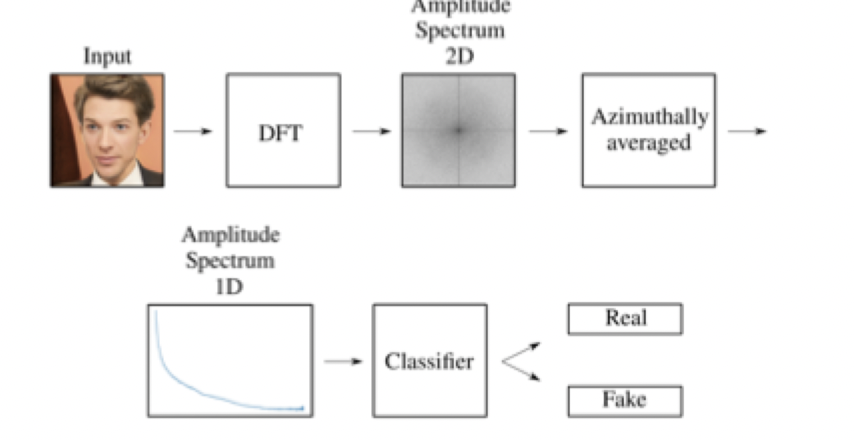
\includegraphics[width=200px]{imgs/Screenshot 2023-12-29 at 12.45.10 AM.png}
    \caption{DFT Pipeline used in \cite{unmasking} and \cite{deepfake-spatio}}
    \label{fig:enter-label}
    \end{center}
\end{figure}


A different but related method for deepfake detection uses Discrete Cosine Transform (DCT), such as in \cite{dct-patchlevel, fighting-dct, lev-freq-dct}. DCT is similar to DFT however, DFT operates on complex numbers while DCT operates on real numbers. DCT is also known to be fast and more effective for image enhancement techniques \cite{dct-review} and JPEG compression. The study by \cite{fighting-dct} used a DCT-blocked based approach to detect GAN Specific Frequencies (GSF) on different GAN-generated images. Their study compiled images from various GAN generators including StarGAN, StyleGAN, and StyleGAN2 and achieved 99.9\%, 100\%, 100\% in accuracy for classifying each respective dataset. These GAN artifacts were also previously studied by \cite{lev-freq-dct} by using DCT. Their study reveals that GAN artifacts are structurally distinguishable by high frequency components in the power spectra. Wavelet Transform was also utilized in studies by \cite{dwt} and \cite{dwt2}. Their study addressed the limitation of using DCT by analyzing images on multi-level frequencies. Like similar studies, however, their dataset only comprised of using GAN-generated faces, limiting the generalizability of their detection method in other object classes.

				
				
		


\section{METHODOLOGY}
\subsection{Data Gathering}

The synthetic images dataset used in this study is from \cite{artifact-dataset} which collated 2,496,738 images, of which 964,989 are classified as real images and 1,531,749 fake images. The fake images in their dataset are generated from different GAN models such as GauGAN, ProGAN, Projected GAN, StarGAN, StyleGAN, StyleGAN2 and StyleGAN3. ProGAN was selected as the dataset for this study due to its wide selection of object classes. The ProGAN images are also available in Nvidia's official website and documentation \citep{progan-nvidia} with dimensions of 256x256, however, the images from Rahman et al.'s study are already narrowed down to 1000 images out of Nvidia's 100,000 generated images per object class. The ProGAN dataset was further classified into 20 classes which are (1) airplane, (2) bicycle, (3) bird, (4) boat, (5) bottle, (6) bus, (7) car, (8) cat, (9) chair, (10) cow, (11) dining table, (12) dog, (13) horse, (14) motorbike, (15) person, (16) plant, (17) sheep, (18) sofa, (19) train, and (20) tv monitor. The real images used for this study comes from the Pascal Visual Object Classes (VOC) Challenge 2012 dataset \citep{pascal-voc-2012}, which also collated images of the same 20 object classes found in the ProGAN dataset. This dataset is originally used for Pascal's image classification and detection challenge. However, since the images from this dataset are collected from 2007-2012, it can be used as a basis for real images. 

For the purpose of this study, only a subset of each dataset will be used for the image classification problem. 200 fake images from the ProGAN dataset and 200 real images from the VOC dataset will be used per object class to train and test the SVM model. This will yield to a total of 8000 images which consists of 4000 fake images and 4000 real images. This is further divided into 60\% for training, and 40\% for testing. Lastly, each image will be resized to a dimension of 200x200 for feature extraction. This dimension is selected for the purpose of easier image slicing for feature extraction. The sample images from the datasets are seen in Figures 2 and 3. 

\begin{figure}[ht]
    \centering
    \vspace{4ex}
	\includegraphics[width=200px]{imgs/fake_imgs.png}
    \caption{Fake images from the ProGAN dataset}
    \label{fig:enter-label}
\end{figure}

\begin{figure}[ht]
    \centering
    \vspace{4ex}
	\includegraphics[width=200px]{imgs/real_img.png}
    \caption{Real images from the Pascal VOC dataset}
    \label{fig:enter-label}
\end{figure}

\subsection{Discrete Cosine Transform}
The Discrete Cosine Transform (DCT) is a sinusoidal transformation based on the Fourier Transform that represents an image as a sum of varying cosine waves. Unlike Discrete Fourier Transform (DFT), DCT operates on real values, whereas DFT uses complex numbers. DCT is also shown to have high energy compaction \citep{dct-energy-compaction}, which allows it to represent more signal information in its coefficients. DCT is used in image enhancements and lossy compression algorithms used in JPEGs. It can also be used for converting images into their frequency domain through a mathematical transformation that allows image compression by determining which values in the DCT coefficient matrix are pertinent in preserving the quality of the image. Typically, during image compression, DCT coefficients with values close to zero are discarded in the computation of the reconstructed image. These lower values are usually found in the high frequency spectrum and do not contribute as much as the low frequency components. However, in GAN-generated images, these components tend to have a relatively higher value as compared to natural or real images. 


DCT was used in studies by \cite{lev-freq-dct} and \cite{fighting-dct} in detecting GAN images for their ability to decompose images into their spectral representation by using the log function. Frank et al. ascertained that GAN images have high frequency components mainly attributed to the architecture of their neural networks. The mathematical equation implemented in SciPy for the 2-dimensional DCT is as follows:

\begin{figure}[ht]
    \centering
    \setkeys{Gin}{width=0.6\textwidth}
    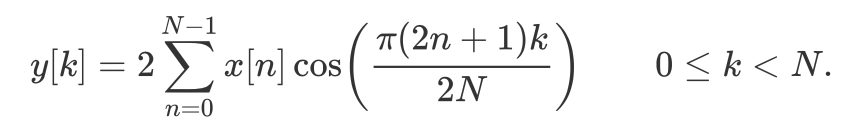
\includegraphics{imgs/formula.png}
\end{figure}

wherein the DCT coefficient y[\textit{k}] will be multiplied by this factor during normalization:

\begin{figure}[ht]
    \centering
    \setkeys{Gin}{width=0.35\textwidth}
    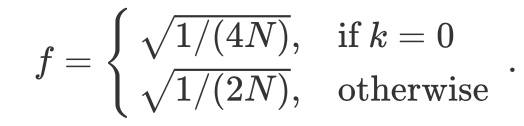
\includegraphics{imgs/factor.png}
\end{figure}


\subsection{Discrete Wavelet Transform}
Discrete Wavelet Transform (DWT) can also be applied to images to decompose them into multiple sub band coefficients. This transformation allows image pixels to be converted into wavelets which can then be used for compression algorithms. Studies by Tang et al. and Liu et al. used wavelet transformation algorithms to address the limitations of analyzing a single frequency spectrum, such as the ones used in DCT. In their studies, DWT was used to analyze the frequency of images in each channel of the RGB color space.

Two Dimensional DWT works by horizontal and vertical filtering of images (treated as a signal) using a high pass and a low pass filter \citep{dwt-method}. This yields to the low-level frequency approximation of the image and its high-frequency details. Each decomposition level divides the image into 4 sub-images, which means that a higher decomposition level would lead to more coefficients. For the purpose of this study, only Level-1 decomposition will be used to extract the DWT coefficients.

\begin{figure}[ht]
    \centering
    \vspace{4ex}
	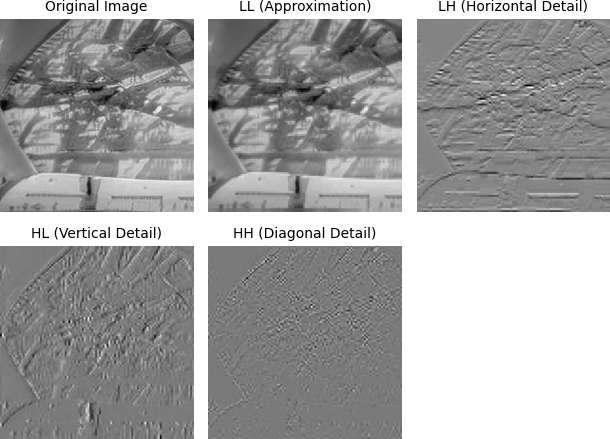
\includegraphics[width=200px]{imgs/img001002_dwt.png}
    \caption{Image decomposition using DWT}
    \label{fig:enter-label}
\end{figure}

\subsection{Feature Extraction}
Obtaining features from images has its own challenges due to their dimensionality. However, we can simplify this through additional image processing steps aimed at extracting numerical features. These features can subsequently be used as input for the classification model.
Before extracting features from real and fake images, two (2) pre-processing methods will be employed separately.

\subsubsection{Discrete Cosine Transform Features}
After reading the images from the dataset and converting them to grayscale, DCT was applied using Scipy's Legacy discrete Fourier transforms' sub-module which includes a method for 2D DCT. The images were then log-transformed for better visualization of image features. The equation for log-transformation is shown in Eq. 1, where  \(I^T(x,y)\) represents the DCT coefficients in the image. After getting the logarithmic representation of the DCT coefficients, the resulting matrix was sliced into non-overlapping blocks with dimensions of 20x20. Since getting all of the DCT coefficients for the input image can lead to over-fitting, each block was averaged to get the floating point features for the SVM model. An image with dimensions of 200 x 200 resulted into 100 features. The definite size of the block took trial and error in an attempt to improve the accuracy of the classifier. Various methods for measuring image noise was also employed, however, it is found that getting the mean values for each block led to a better accuracy for the SVM classifier. The DCT pipeline can be seen in Figure 5. 

\begin{equation}
    I_{log}(x,y) = \ln(|I^{T}(x,y) | + 1)
\end{equation}

\subsubsection{Discrete Wavelet Transform Features}
Applying level-1 Haar Wavelet Transform on the images yielded to 4 sub-images which holds the values for the LL (low-level approximation), LH (horizontal detail), HL (vertical detail), and HH (diagonal detail) coefficients (Fig. 4). Since most GAN architectures make use of a random noise as an input to create fake images, it is hypothesized that GAN-generated images contain higher values of noise as compared to real ones. A study by \cite{dwt-noise}  on image noise estimation using DWT found that the majority of coefficients corresponding to noise are found in the HH sub-band. However, including the rest of the DWT coefficients led to a better discriminatory performance for the classifier. The first feature that was considered for the DWT images was entropy. Entropy is the measure of randomness in the pixel values of the image, which can also be used to measure variability in the DWT sub-images. Shannon entropy can be computed using the mathematical formula in Eq. 2. Statistical features to measure variability and noise distribution in images such as mean, variance and standard deviation was also used. Lastly, blobs using the Difference of Gaussian (DoG) method was counted and extracted as image features. DoG is used in image enhancement and edge detection, however it can also be used for removal of random noise in images \citep{DoG}. It suppresses high frequency components from the image by using a Gaussian filter to create heavily blurred images and subtracting it from a less blurred version of the same image. The list of features and pipeline used for DWT is seen in Figure 6. 

\begin{equation}
   H = − \sum _{i=0}^{L-1}p_{i} log_{2}(p_{i})
\end{equation}

Additionally, entropy was also measured from both raw images before applying image transformation. Since GAN-generated images are trained on numerous image sets, it is hypothesized that synthetic images would have higher variability as compared to real images. Each of the features used for the model resulted to a single floating point value, which will be fed to the SVM model for classification. 

\begin{figure}[ht]
\begin{center}
    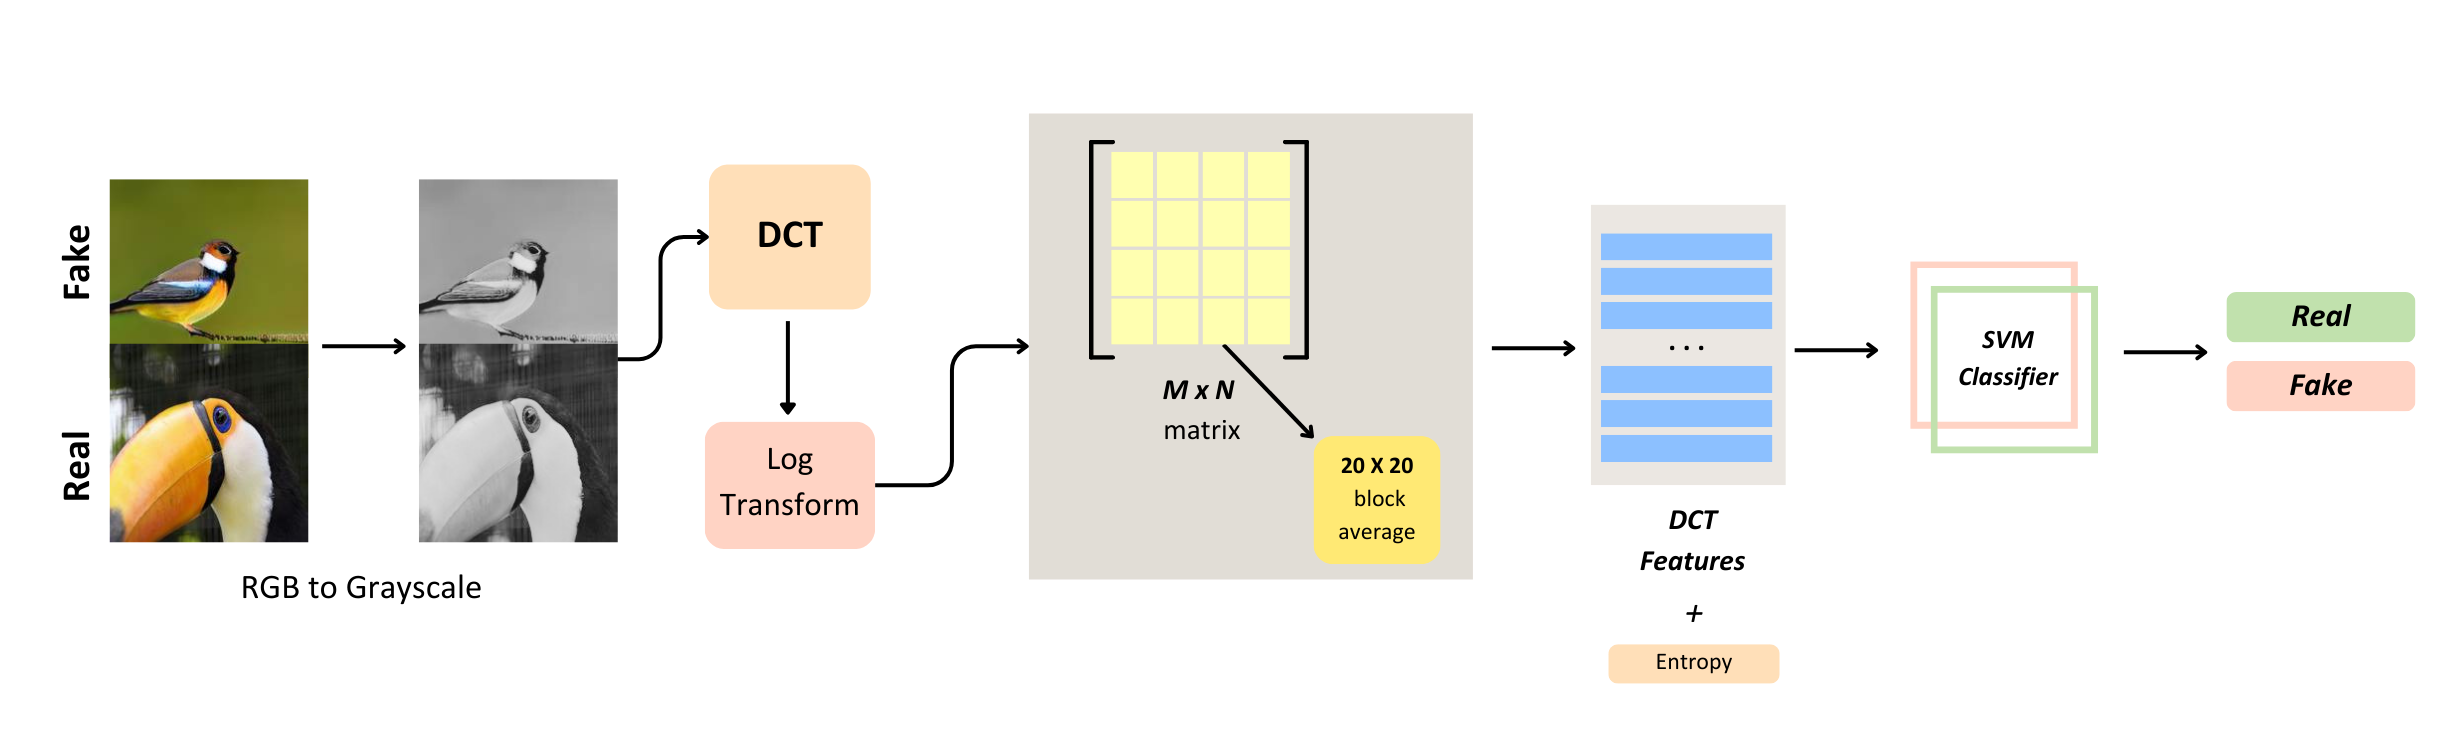
\includegraphics[width=440px,height=4cm]{imgs/1.png}
    \caption{DCT Pipeline}
    \label{Fig:image label}
\end{center}
\end{figure}

\begin{figure}[ht]
\begin{center}
    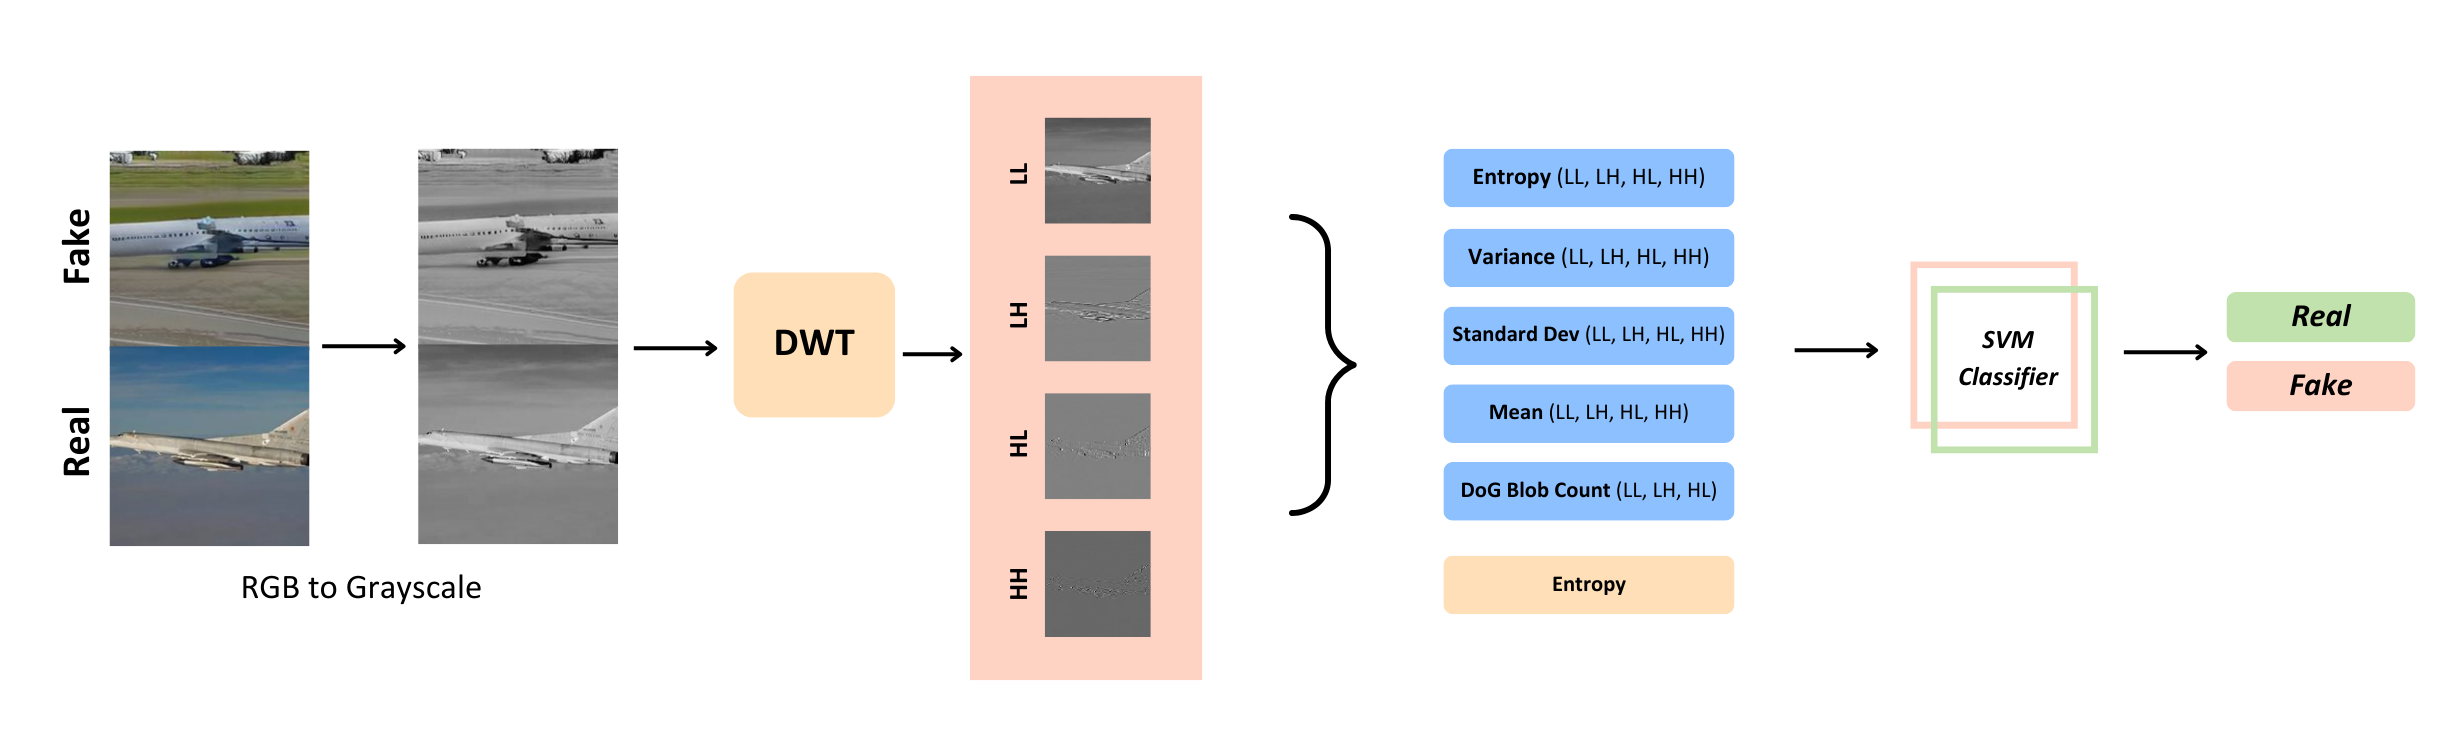
\includegraphics[width=440px,height=4cm]{imgs/2.png}
    \caption{DWT Pipeline}
    \label{Fig:image label}
\end{center}
\end{figure}

%refine this section
\subsection{Support Vector Machine Model}
A Support Vector Machine (SVM) was built to classify image features gathered from the two pre-processing methods. All of the features used in this classification problem have a numerical data type for simplification. For binary classification, SVM is proven to be effective in handling high-dimensional data, which is useful considering that DCT images have a total of 101 features, and DWT images have 20 features. Additionally, a test for combining these methods would yield to a total of 120 features (note that entropy was used for both DCT and DWT). The SVM model was built using a Radial Basis Function (RBF) kernel to make a substantial margin between the two classification groups. Different hyper-parameters were also used for each pre-processing method. Using grid search, it was found that using the DCT features, the best C and gamma ($\gamma$) value would be 10 and 0.01. Using DWT features, the optimal values were C = 100, and  $\gamma$ = 0.01. 10-fold cross validation was also done to check the model for over-fitting.  

\subsection{Language and Libraries}
Python will be used as the programming language for this study. It is a high-level interpreted language that offers numerous open-source libraries which can be used for the statistical analysis and image operations. SciPy, a broadly applicable and open source library, will be used to perform DCT on the images. DWT on the other hand will be performed using PyWavelet. Since images are interpreted as matrices of pixel values, Numpy will be used for computation alongside Matplotlib for data visualization. Scikit will also be used to build and train the SVM model. Scikit is a machine learning library for Python that offers different classification, regression and clustering algorithms. Lastly, to develop a Graphical User Interface (GUI) for this classification problem, Tkinter, Python’s native framework, will be used.

\subsection{Evaluation Metrics}
The primary objective of this study is to determine whether GAN traces in the frequency domain exist even in various object classes. By applying Discrete Cosine Transform (DCT) and Discrete Wavelet Transform (DWT) as distinct pre-processing methods on the images, their accuracy will be measured to evaluate how well these methods work as a way to identify GAN-generated images. For binary classification, a confusion matrix is deemed useful to visualize the SVM model's accuracy in classifying the testing data vis-a-vis the proposed methods. Additionally, cross-validation accuracy will be computed to assess the robustness and generalizability of the proposed methods in classifying images across the datasets.




		
\section{RESULTS AND DISCUSSION}
The SVM model was used to classify fake and real images on the ProGAN and VOC dataset. These images were spread across various object classes to determine the generalizability of the proposed methods on detecting GAN-generated images. In order to evaluate how well the extracted features using DCT and DWT are able to discriminate fake and real images in the frequency domain, accuracy was measured. The initial testing for both DCT and DWT features were first conducted and measured across the entire dataset. This still followed the 40\% data for testing and 60\% for training. Cross validation was done across the entire dataset to measure the features' robustness across all collected images. The results of the initial testing are summarized in Table 1. It should be noted that the 20 x 20 slice dimension was used for the DCT features. Furthermore, the features for both DCT and DWT consisted of the 100 DCT slice mean, DWT entropy, variance, standard deviation, mean, and blob count. Entropy from the raw image was also considered as additional feature for both DCT and DWT. 
\\
%table for initial testing
\begin{table}[H]
\centering
\begin{tabular}{|c|c|c|c|c|}
\hline
Method    & Accuracy & CV Mean Accuracy & C   & $\gamma$    \\ \hline
DCT       & 97.1875  & 97.2375          & 10  & 0.01 \\ \hline
DWT       & 79.0313  & 68.8125          & 100 & 0.01 \\ \hline
DCT + DWT & 97.0313  & 92.7624          & 10  & 0.01 \\ \hline
\end{tabular}
\caption{Initial Testing Results}
\end{table}

During initial testing, it was found that the average of the DCT coefficients were adequate to discriminate from fake or real images. This is because DCT coefficients are useful determinants of noise presence in images \citep{noise-estimation}. Since GAN-generated images are created from random noise, we can inspect images in the frequency domain and discriminate them using DCT features. The study \cite{lev-freq-dct} also used the coefficients from DCT as their features for GAN image classification, however, in their study all of the matrix coefficients were taken into account. Using the image dimensions of 200 x 200, this would yield to 40,000 features which would be very complex for a simple classifier. Even if SVM is able to handle high dimensional data, the risk for over-fitting is still present and so finding a good balance for the number of features without sacrificing accuracy poses a challenge. Table 2 suggests that a slice size of 20x20 provides the best accuracy and cross validation mean accuracy among all slices with a total of 100 features for the SVM model. 

\\
%Tables and figures for DCT slice size
\begin{table}[H]
\centering
\begin{tabular}{|c|c|c|c|c|c|}
\hline
\textit{\textbf{N}} & Accuracy         & CV Mean Accuracy & C           & γ             & Features     \\ \hline
8                   & 96.9063          & 96.975           & 10          & 0.001         & 625          \\ \hline
10                  & 96.9688          & 96.9875          & 10          & 0.001         & 400          \\ \hline
\textbf{20}                  & \textbf{97.1875} & \textbf{97.2375} & \textbf{10} & \textbf{0.01} & \textbf{100} \\ \hline
25                  & 96.8438          & 97.00            & 10          & 0.01          & 64           \\ \hline
40                  & 97.0938          & 96.825           & 100         & 0.01          & 25           \\ \hline
50                  & 96.2188          & 96.1             & 100         & 0.01          & 16           \\ \hline
100                 & 75.4375          & 75.125           & 1           & 1             & 4            \\ \hline
200                 & 60.25            & 60.3625          & 1           & 1             & 1            \\ \hline
\end{tabular}
\caption{DCT Slices Initial Testing Results}
\end{table}

\begin{figure}[ht]
    \centering
   \vspace{4ex}
	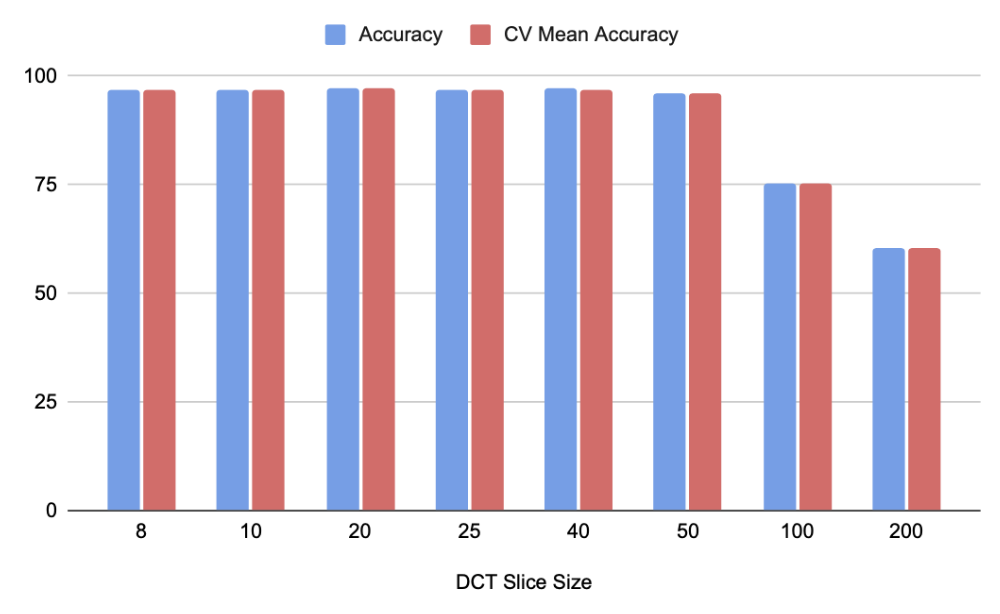
\includegraphics[width=200px]{imgs/Acc_slize.png}
    \caption{DCT Accuracy vs Slice Size}
    \label{fig:enter-label}
\end{figure}


During initial testing, it was concluded that the slicing method used for DCT is not very useful for extracting DWT features. However, various decomposition level for DWT was tested using the features selected above and the results are shown in Table 3. 
%Tables and figures for DWT levels
\begin{table}[ht]
\centering
\begin{tabular}{|c|c|c|c|c|c|}
\hline
DWT Level  & Accuracy         & CV Mean Accuracy & Image Size         & C            &  $\gamma$          \\ \hline
\textbf{1} & \textbf{79.0313} & \textbf{68.8125} & \textbf{100 x 100} & \textbf{100} & \textbf{0.01} \\ \hline
2          & 66.0937          & 59.25            & 50 x 50            & 1            & 0.1           \\ \hline
3          & 67.0313          & 65.5             & 25 x 25            & 100          & 0.01          \\ \hline
\end{tabular}
\caption{DWT Decomposition Level Initial Testing Results}
\end{table}

\begin{figure}[ht]
    \centering
    \vspace{4ex}
	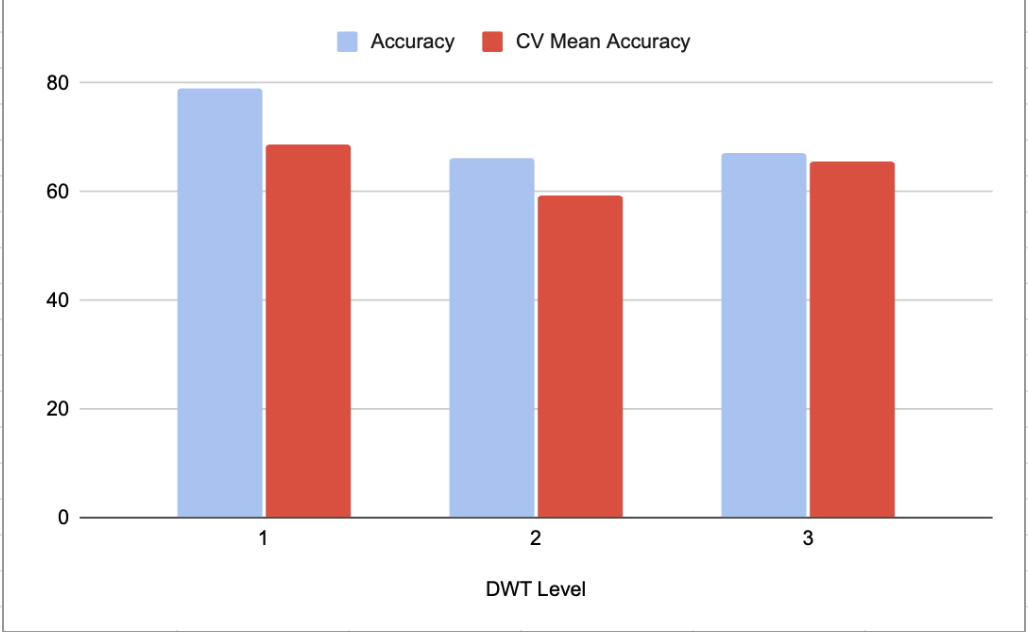
\includegraphics[width=200px]{imgs/dwt_level.png}
    \caption{DWT Accuracy vs Decomposition Level}
    \label{fig:enter-label}
\end{figure}

From Table 3, we can see that using the DWT features was not very effective in classifying fake from real images as compared to using DCT features. We can also see that using a higher level of decomposition using the same features would yield to a lower performance for the classifier. This can be attributed to the image compression that happens for every decomposition level. Using level-\textit{L} DWT would yield to 4 sub-images with dimensions equal to \( \frac{M}{2^L} \) x \( \frac{N}{2^L} \), where \textit{M} and \textit{N} are the image width and height and L represents the decomposition level.


After initial testing, and the features for both DCT and DWT were finalized, the images for testing and training were randomly selected from the dataset to extract their features for the SVM model and the desktop application. The training data consisted of 4800 randomly selected images from various object classes, while the training data was further split into 2400 images for the SVM model and 800 images for image prediction using the desktop application. The DCT and DWT features for both the testing and training data were stored in separate CSV files, facilitating easier loading. Their accuracies are measured and shown in Table 4. 

\\
%table for final accuracies
\begin{table}[H]
\centering
\begin{tabular}{|c|c|c|c|}
\hline
Method             & Accuracy        & C            & $\gamma$            \\ \hline
DCT                & 97.0833         & 10           & 0.01           \\ \hline
DWT                & 79.8333         & 100          & 0.01           \\ \hline
\textbf{DCT + DWT} & \textbf{97.125} & \textbf{100} & \textbf{0.001} \\ \hline
\end{tabular}
\caption{Final Testing Results}
\end{table}

%%begin conf mat
\begin{figure*}
    \centering
    \vspace{4ex}
    \subfloat[DCT]{
        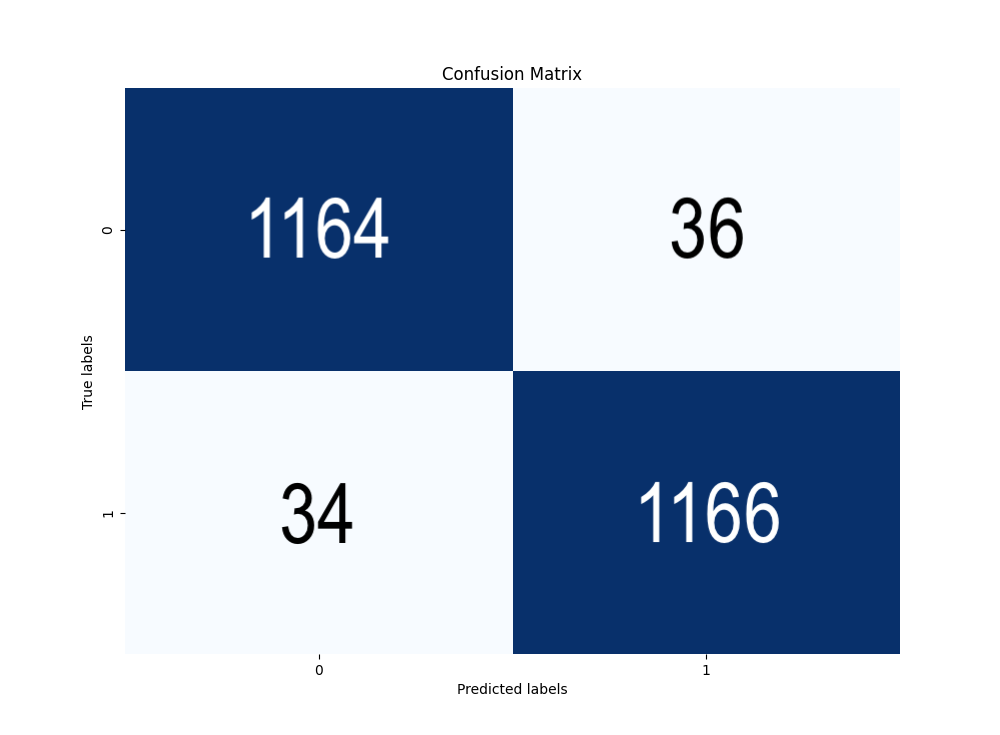
\includegraphics[width=0.3\linewidth]{imgs/DCT_conf_mat.png}
        \label{fig:subfig1}
    }
    \hfil
    \subfloat[DWT]{
        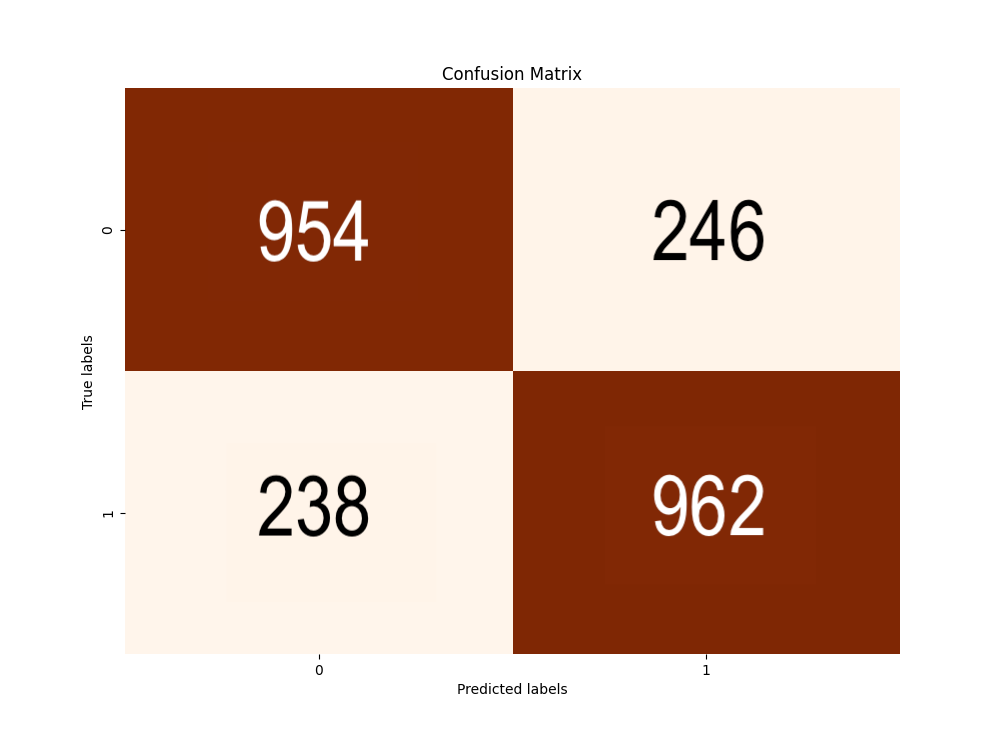
\includegraphics[width=0.3\linewidth]{imgs/DWT_conf_mat.png}
        \label{fig:subfig2}
    }
    \hfil
    \subfloat[DCT+DWT]{
        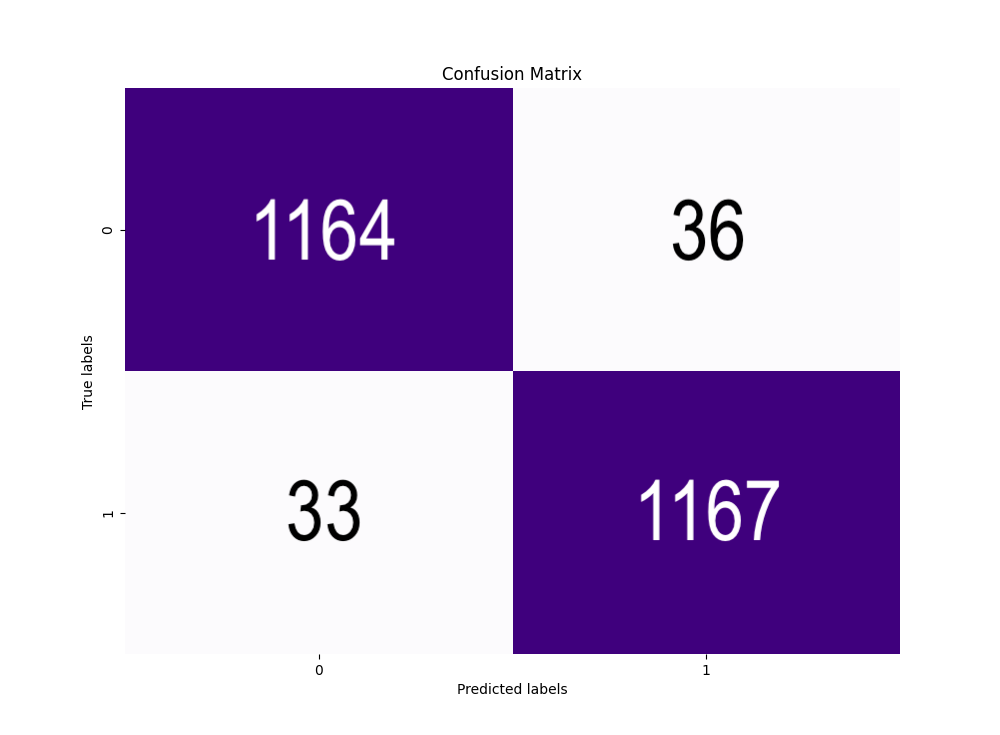
\includegraphics[width=0.3\linewidth]{imgs/BOTH_conf_mat.png}
        \label{fig:subfig3}
    }
    \caption{Confusion Matrices Using Each Method}
    \label{fig:mainfig}
\end{figure*}
%%end conf mat

\\
\begin{table}[ht]
\centering
\begin{tabular}{|c|c|c|c|c|}
\hline
Method                                                               & Class & Precision       & Recall          & F1-Score        \\ \hline
\multirow{2}{*}{DCT}                                                 & Real  & 0.9716          & 0.9700          & 0.9708          \\ \cline{2-5} 
                                                                     & Fake  & 0.9700          & 0.9717          & 0.9709          \\ \hline
\multirow{2}{*}{DWT}                                                 & Real  & 0.8003          & 0.7950          & 0.7977          \\ \cline{2-5} 
                                                                     & Fake  & 0.7964          & 0.8017          & 0.7990          \\ \hline
\multirow{2}{*}{\begin{tabular}[c]{@{}c@{}}DCT +\\ DWT\end{tabular}} & Real  & \textbf{0.9724} & \textbf{0.9700} & \textbf{0.9712} \\ \cline{2-5} 
                                                                     & Fake  & \textbf{0.9701} & \textbf{0.9725} & \textbf{0.9713} \\ \hline
\end{tabular}
\caption{Additional Evaluation Metrics}
\end{table}

Table 5 suggests that using both DCT and DWT features yield to a better classification performance, however, it is not a significant difference from using DCT alone. The confusion matrices for the employed methods are also seen in Figure 9. Additional evaluation metrics such as precision, recall, and F1-score are also highlighted in Table 5. From these metrics, we can observe that precision, recall, and f1-score are highest when using both DCT and DWT features. However, similar to accuracy, their values are not significantly higher than using DCT features alone.  

\begin{figure}[ht]
    \centering
    \vspace{4ex}
	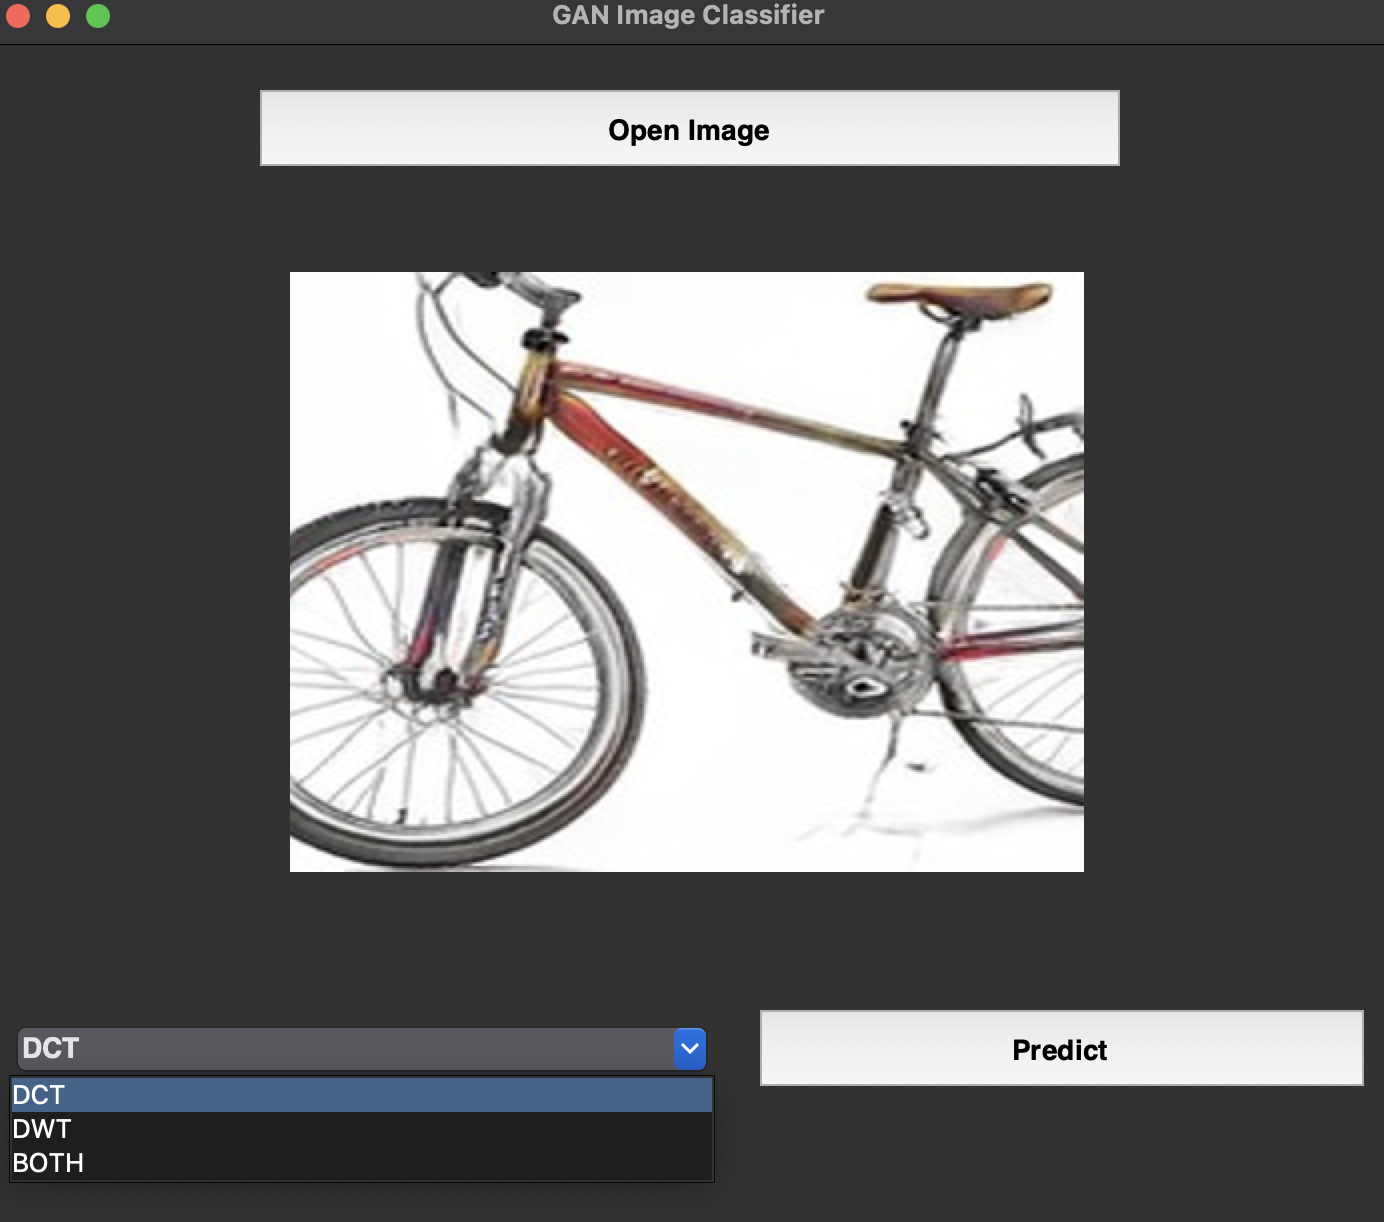
\includegraphics[width=400px]{imgs/app.png}
    \caption{Application Interface with Method Selection}
    \label{fig:enter-label}
\end{figure}

To further test the SVM classifier vis-a-vis the proposed methods, a Graphical User Interface was developed (See Fig. 10). This allows users to select an image from a dataset, and determine whether it is fake or real using the following methods: DCT, DWT, and BOTH. The selected image will first be resized (if it does not follow the 200x200 dimension) before passing it to the DCT and/or DWT feature extractor. This would yield to a CSV file containing pertinent features which the SVM model will predict. Additional testing using images from the StyleGAN2 dataset and some images collected from the internet were used in the application. Their results along with the methods used for detection are seen in the following figures. 

%progan images
\begin{figure*}
    \centering
    \subfloat[DCT]{
        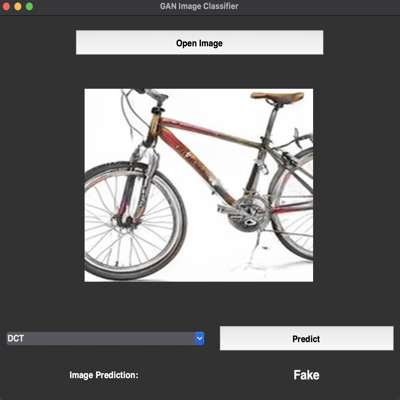
\includegraphics[width=0.3\linewidth]{imgs/preds/pg-f1.png}
        \label{fig:subfig1}
    }
    \hfil
    \subfloat[DWT]{
        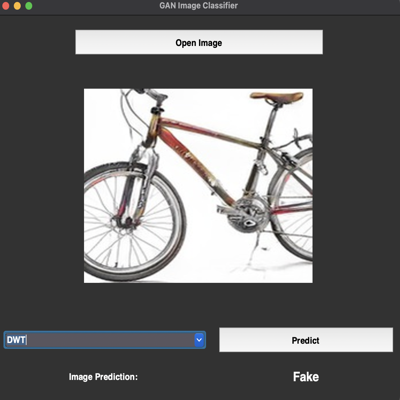
\includegraphics[width=0.3\linewidth]{imgs/preds/pg-f2.png}
        \label{fig:subfig2}
    }
    \hfil
    \subfloat[DCT+DWT]{
        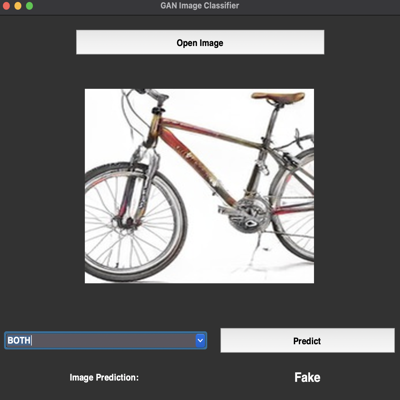
\includegraphics[width=0.3\linewidth]{imgs/preds/pg-f3.png}
        \label{fig:subfig3}
    }
    \caption{Fake Image From the ProGAN Dataset Detected as Fake}
    \label{fig:mainfig}
\end{figure*}

\begin{figure*}
    \centering
    \subfloat[DCT]{
        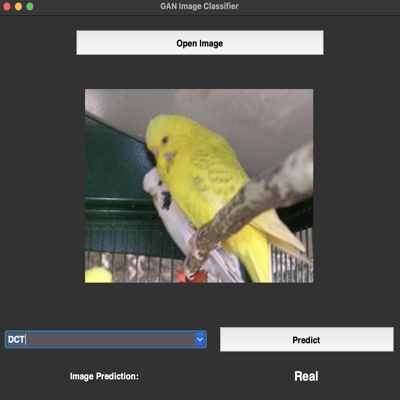
\includegraphics[width=0.3\linewidth]{imgs/preds/pg-r3.png}
        \label{fig:subfig1}
    }
    \hfil
    \subfloat[DWT]{
        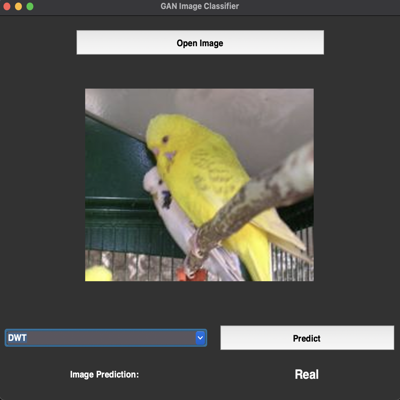
\includegraphics[width=0.3\linewidth]{imgs/preds/pg-r2.png}
        \label{fig:subfig2}
    }
    \hfil
    \subfloat[DCT+DWT]{
        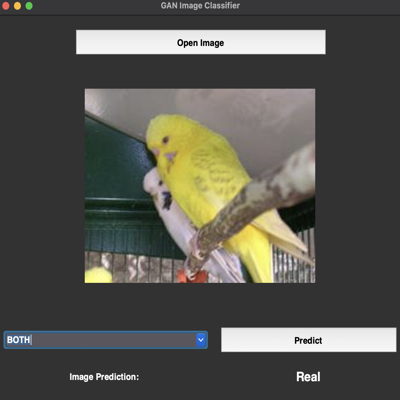
\includegraphics[width=0.3\linewidth]{imgs/preds/pg-r1.png}
        \label{fig:subfig3}
    }
    \caption{Real Image From the VOC Dataset Detected as Real}
    \label{fig:mainfig}
\end{figure*}

%stylegan images
\begin{figure*}
    \centering
    \subfloat[DCT]{
        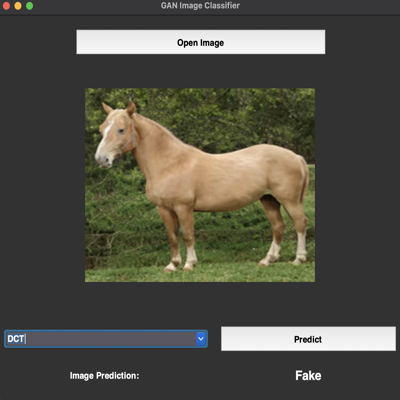
\includegraphics[width=0.3\linewidth]{imgs/preds/sg-f1.png}
        \label{fig:subfig1}
    }
    \hfil
    \subfloat[DWT]{
        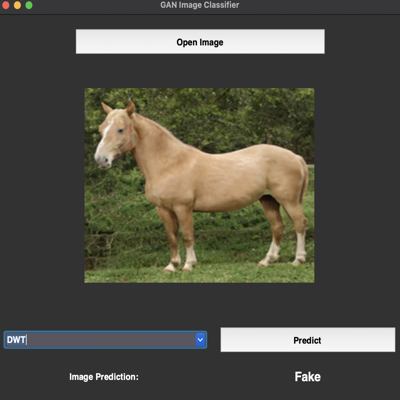
\includegraphics[width=0.3\linewidth]{imgs/preds/sg-f2.png}
        \label{fig:subfig2}
    }
    \hfil
    \subfloat[DCT+DWT]{
        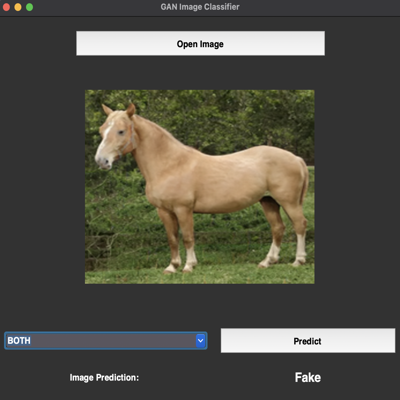
\includegraphics[width=0.3\linewidth]{imgs/preds/sg-f3.png}
        \label{fig:subfig3}
    }
    \caption{Fake Image From the StyleGAN2 Dataset Detected as Fake}
    \label{fig:mainfig}
\end{figure*}



Figures 11 and 12 demonstrate the identification of the fake and real images from the ProGAN dataset. Even if DWT has a lower accuracy as compared to DCT and using both DCT+DWT, it was still able to correctly identify most of the images. Additional testing using the images from the StyleGAN2 dataset was also conducted. From Figures 13-14 we can see that even if it was not trained on the StyleGAN2 dataset, it was able to correctly identify which images are real or fake. Further testing using images gathered from the Internet through Google Images was conducted to test the performance of the proposed methods. Figures 15-16 show the results of the classifier using DCT, DWT, and both methods. Figure 16-b demonstrates the misclassification of a real image using the DWT method alone. However, DCT and both DCT+DWT features were able to correctly classify the given image.





\begin{figure*}
    \centering
    \subfloat[DCT]{
        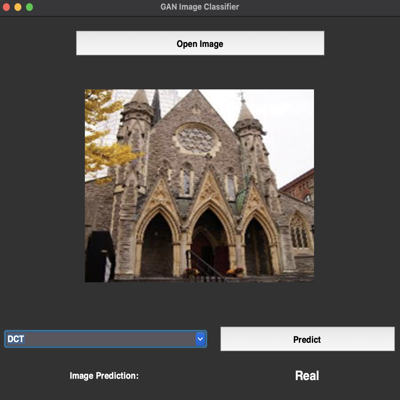
\includegraphics[width=0.3\linewidth]{imgs/preds/sg-r3.png}
        \label{fig:subfig1}
    }
    \hfil
    \subfloat[DWT]{
        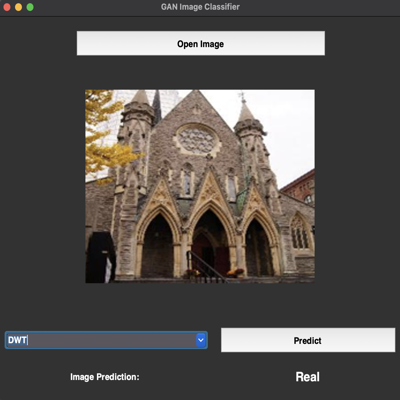
\includegraphics[width=0.3\linewidth]{imgs/preds/sg-r2.png}
        \label{fig:subfig2}
    }
    \hfil
    \subfloat[DCT+DWT]{
        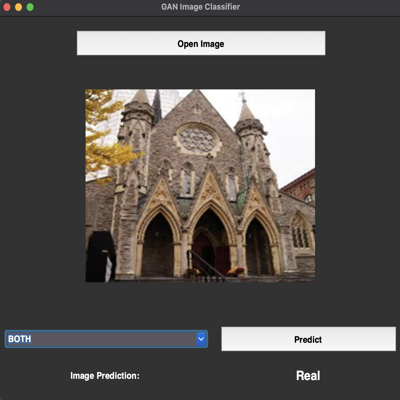
\includegraphics[width=0.3\linewidth]{imgs/preds/sg-r1.png}
        \label{fig:subfig3}
    }
    \caption{Real Image From the StyleGAN2 Dataset Detected as Real}
    \label{fig:mainfig}
\end{figure*}

%internet images
\begin{figure*}
    \centering
    \subfloat[DCT]{
        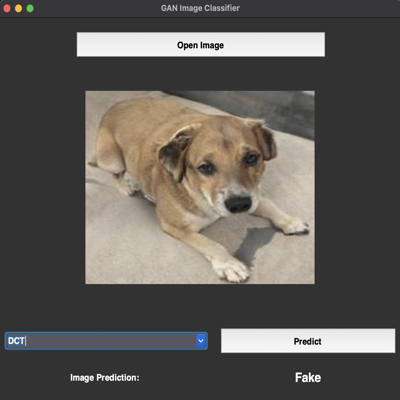
\includegraphics[width=0.3\linewidth]{imgs/preds/i-f1.png}
        \label{fig:subfig1}
    }
    \hfil
    \subfloat[DWT]{
        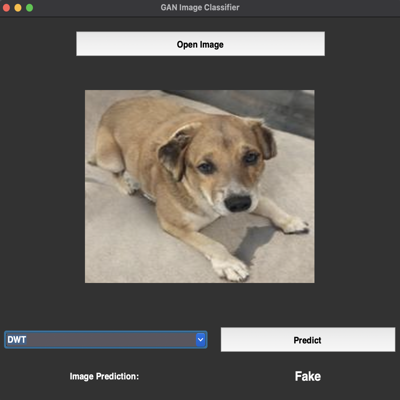
\includegraphics[width=0.3\linewidth]{imgs/preds/i-f2.png}
        \label{fig:subfig2}
    }
    \hfil
    \subfloat[DCT+DWT]{
        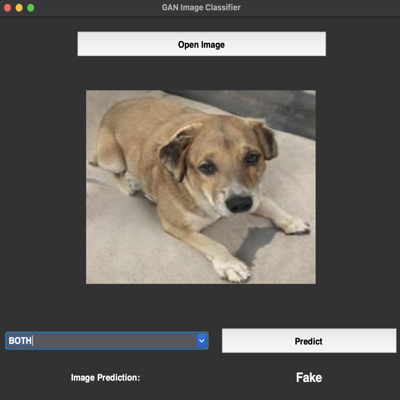
\includegraphics[width=0.3\linewidth]{imgs/preds/i-f3.png}
        \label{fig:subfig3}
    }
    \caption{Fake Image Download From the Internet Dataset Detected as Fake}
    \label{fig:mainfig}
\end{figure*}

\begin{figure*}
    \centering
    \subfloat[DCT]{
        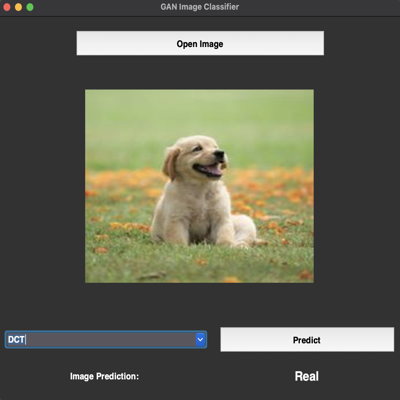
\includegraphics[width=0.3\linewidth]{imgs/preds/i-r3.png}
        \label{fig:subfig1}
    }
    \hfil
    \subfloat[Misclassified DWT]{
        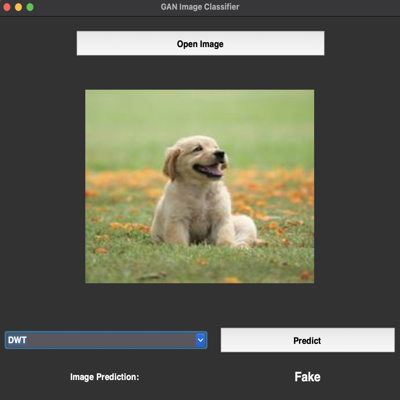
\includegraphics[width=0.3\linewidth]{imgs/preds/i-r2.png}
        \label{fig:subfig2}
    }
    \hfil
    \subfloat[DCT+DWT]{
        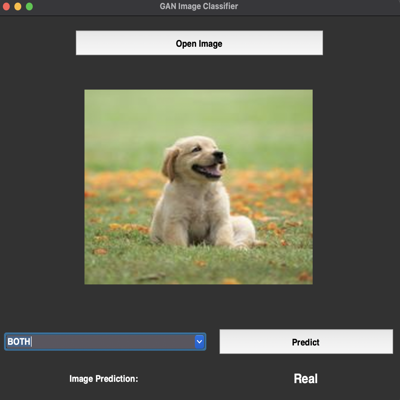
\includegraphics[width=0.3\linewidth]{imgs/preds/i-r1.png}
        \label{fig:subfig3}
    }
    \caption{Real Image Downloaded From the Internet Dataset Detected as Real}
    \label{fig:mainfig}
\end{figure*}
		

\section{SUMMARY AND CONCLUSION}
This study demonstrated how GAN-generated images have discernible features in the frequency domain. By exploiting transformation methods such as Discrete Cosine Transform and Discrete Wavelet Transform to convert images into their frequency domain, we can extract useful features which can be used for classification. Furthermore, we can see that these features are generalizable across various object classes. This study found out that even simple features such as the mean of DCT coefficient slices are informative factors for GAN image classification. This is due to DCT's ability to measure the distribution of energy levels which can be used to capture GAN-specific frequencies.  

For future studies, it is worth investigating other methods to improve the accuracy of using DWT features. Another recommendation would be to try out other datasets from different GAN architectures with various object classes to see if using DCT or DWT would be useful in identifying GAN-generated images. Future studies could also investigate how the classifier or feature extraction method works for various image dimensions. Lastly, to determine the robustness of using DCT features for GAN image classification, future studies could look into testing for common image perturbations to determine the proposed method's performance against adversarial attacks. 


%\section{Recommendation}


% APPENDICES
\appendices

\section{ADDITIONAL TESTING ON OTHER GAN ARCHITECTURES}
To further validate the performance of the DCT method in identifying GAN-generated images, 25 'fake' images were collected from 5 different GAN architectures namely (1) Big GAN, (2) Cycle GAN, (3) Difussion GAN, (4) Gau GAN, and (5) Projected GAN. Feature extraction through DCT was done per architecture and their results using the SVM model trained on the ProGAN features are seen in Table 6.

\begin{table}[H]
\centering
\begin{tabular}{|c|c|c|}
\hline
GAN           & Classified Correctly & Accuracy \\ \hline
Big GAN       & 19/25                & 76\%     \\ \hline
Cycle GAN     & 21/25                & 84\%     \\ \hline
Diffusion GAN & 5/25                 & 20\%     \\ \hline
Gau GAN       & 21/25                & 84\%     \\ \hline
Projected GAN & 16/25                & 64\%     \\ \hline
\end{tabular}
\end{table}


Although being trained using the ProGAN images, the model was able to perform well on classifying GAN images generated from Big Gan, Cycle GAN, and Gau GAN. However, we can see it poorly perform on classifying images generated using the Diffusion GAN. Upon further research, it was found that the main difference of the diffusion model as compared to other GAN architectures is the way it generates images. Diffusion GANs create images through noise insertion and incrementally denoising the image to reconstruct it. This process of iterative denoising could be the reason why it slips through the DCT method, which exploits the noise property of GAN-generated images. 
		
  
  %References command
		%Parameter is the references bib file without extension
		\makereferences{references}
			
	\end{mainmatter}
\end{document}
